% siminos/kittens/prime.tex  % pdflatex CL18.tex
% $Author: predrag $ $Date: 2020-10-04 12:43:42 -0400 (Sun, 04 Oct 2020) $


\section{Enumeration of prime \twots}
\label{s:prime}
% Predrag                                       2020-08-12
% extracted from siminos/spatiotemp/chapter/prime.tex  (a blogCats.tex section)
% former \label{sect:Count2dprimePO}
% the two are now edited separately

Here we show how to enumerate the total numbers of distinct periodic states
in terms of prime \twots.

The enumeration of \catlatt\ doubly-periodic lattice states proceeds in 3
steps:
\begin{enumerate}
  \item
Construct a hierarchy of 2\dmn\ Bravais lattices $\Lambda$, starting with
the smallest Bravais cells \refeq{Hermite2d}, list Bravais lattices by
increasing \LTS{}{}{}, one per each set related by discrete symmetries
\refeq{eq:C4v}.
  \item
For each $\Lambda = \LTS{}{}{}$ Bravais lattice, compute $N_\Lambda$, the
number of doubly-periodic \catlatt\ lattice states, using the
`fundamental fact' $N_\Lambda=\left|\det\jMorb(\Lambda)\right|$.
  \item
We have defined the \emph{prime} Bravais lattice in \refsect{s:primeLatt}.
  \item
The total number
of (doubly) periodic
\brick s is the sum of all cyclic permutations of prime \brick s,
\[
N_\Lambda
    %  |\A|^{\speriod{}\period{}}
=
\sum_p N_{p}\,\LTS{p}{p}{p}
\]
where the sum goes over prime tilings of the $\LTS{}{}{}$
\brick.
\end{enumerate}

\PCedit{
The number of prime \twots\ is given recursively by
(see \refeq{primeCount}),
\beq
M_{p}\,=\,\frac{1}{\speriod{}\period{}}
  \left( N_{p}
          - \sum _{p'}
            \speriod{p'}\period{p'}
                                          \, M_{p'}
  \right)
\,,
\ee{primeCount2D}
where the sum is over $p'$, the prime `divisors' of $p$
that satisfy tiling conditions \refeq{primeTiling}.
    }



%%%%%%%%%%%%%%%%%%%%%%%%%%%%%%%%%%%%%%%%%%%%%%%%%%%%%%
% siminos/spatiotemp/tables/LxTs5o2.tex
% $Author: predrag $ $Date: 2021-08-10 11:56:19 -0400 (Tue, 10 Aug 2021) $

%%%%%%%%%%%%%%%%%%%%%%%%%%%%%%%%%%%%%%%%%%%%%%%%%%%%%%
% called by blogCats.tex and CL18.tex
% 2020-06-09 HL siminos/mathematica/PrimeSolutions.nb
%            Edited the tables of numbers of prime solutions
% Predrag 2019-11-23 started with ChaosBook \reftab{tab:primeTwots}
\begin{table}
\caption[]{\label{tab:LxTs=5/2}    \small
The numbers of the ${s}=5/2$ \catlatt\
$\LTS{}{}{}$ \twots: $M_{\LTS{}{}{}}$ is the
number of prime \twots, $N_{\LTS{}{}{}}$ is the
number of doubly periodic {\lattstate}s,
and $R_{\LTS{}{}{}}$ is the number of prime \twots\ in the
$\Dn{4}$ symmetries orbit.
}
\begin{center}
%\renewcommand{\arraystretch}{0.8}
{\small
\begin{tabular}{lrlr}
\\[-16pt]
$\LTS{}{}{}$
                  & $M$ %_{[\speriod{}\!\times\!\period{}]}$
                         & $N$ %_{[\speriod{}\!\times\!\period{}]}$
                                                 &$R$\\
\hline
$\BravCell{1}{1}{0}$  &   1  &   1                   & 1 \\
$\BravCell{2}{1}{0}$  &   2  &
  $5~=\;\;\,2\,\BravCell{2}{1}{0}+1\,\BravCell{1}{1}{0}$
                                                 & 2 \\
$\BravCell{2}{1}{1}$&   4  & 9~\;=\;\;\,$
                           {4}\,\BravCell{2}{1}{1}
                         + {1}\,\BravCell{1}{1}{0}$
                                                 &   \\
$\BravCell{3}{1}{0}$  &   5  & 16 =~ ${5}\,\BravCell{3}{1}{0}
                         + {1}\,\BravCell{1}{1}{0}$
                                                 &   \\
$\BravCell{3}{1}{1}$&   16 & $49 =16\,\BravCell{3}{1}{1}
                         + {1}\,\BravCell{1}{1}{0}$
                                                 &   \\
%$\BravCell{3}{1}{2}$&   16 & $49 =16\,\BravCell{3}{1}{2}  % (49-1)/3
%                         + {1}\,\BravCell{1}{1}{0}$
%                                                 &   \\
$\BravCell{4}{1}{0}$  &  10 & $45 =10\,\BravCell{4}{1}{0} % (45-2*2-1)/4
                         + {2}\,\BravCell{2}{1}{0}
                         + {1}\,\BravCell{1}{1}{0}$
                                                 &   \\
$\BravCell{4}{1}{1}$&   54 & $225 =54\,\BravCell{4}{1}{1} % (225-4*2-1)/4
			+{4}\,\BravCell{2}{1}{1}
                         + {1}\,\BravCell{1}{1}{0}$
                                                 &   \\
$\BravCell{4}{1}{2}$&   60 & $245 =59\,\BravCell{4}{1}{2} % (245-2*2-1)/4
                         + {2}\,\BravCell{2}{1}{0}
                         + {1}\,\BravCell{1}{1}{0}$
                                                 &   \\
%$\BravCell{4}{1}{3}$&   56 & $225 =56\,\BravCell{4}{1}{2}
%                         + {1}\,\BravCell{1}{1}{0}$
%                                                 &   \\
$\BravCell{2}{2}{0}$  &   52  & $225 =
               {52}\,\BravCell{2}{2}{0}
             + {2}\,\BravCell{2}{1}{0}
             + {2}\,\BravCell{1}{2}{0}$
                                                 &   \\
                      &       & $\quad\quad\;\;
             + {4}\,\BravCell{2}{1}{1}
             + {1}\,\BravCell{1}{1}{0}$
                                                 & 1 \\
$\BravCell{2}{2}{1}$&  60 & $245 = 60\,\BravCell{2}{2}{1}  % (245-2*2-1)/4
			+ {2}\,\BravCell{1}{2}{0}
                         + {1}\,\BravCell{1}{1}{0}$
                                                 &   \\
$\BravCell{3}{2}{0}$  & 850  &
                          $ 5\,120 =850\,\BravCell{3}{2}{0}
                          +5\,\BravCell{3}{1}{0}$
                                                 &   \\
                      &       & $\qquad\quad\;\,
                          +2\,\BravCell{1}{2}{0}
                          +1\,\BravCell{1}{1}{0}$
                                                 &   \\
$\BravCell{3}{2}{1}$& 1\,012 &
                           $ 6\,125 =1\,012\,\BravCell{3}{2}{1} %(6125 - 16*3-2*2 -1)/6
                           +16\,\BravCell{3}{1}{2}$
                                                 &   \\
                      &       & $\qquad\quad~~
                           +2\,\BravCell{1}{2}{0}
                           +~\,1\,\BravCell{1}{1}{0}$
                                                 &   \\
%$\BravCell{3}{2}{2}$&      & 6125 =?$\BravCell{3}{2}{2}
%                         + {1}\,\BravCell{1}{1}{0}$
%                                                 &   \\
$\BravCell{3}{3}{0}$  & 68\,281 &

                         $ 614\,656 = 68\,281\,\BravCell{3}{3}{0}
                         +  5\,\BravCell{3}{1}{0}$  %(614656 -2*16*3 - 5*3 - 5*3 -1)/9$
                                                 &   \\
                      &       & $\,
                         + 16\,\BravCell{3}{1}{1} +16 \,\BravCell{3}{1}{2}
                         +  5\,\BravCell{1}{3}{0}
                         + {1}\,\BravCell{1}{1}{0}$
                                                 & 1  \\
$\BravCell{3}{3}{1}$& 70\,400  &
                         $ 633\,616 =70\,400\,\BravCell{3}{3}{1}
                         + {5}\,\BravCell{1}{3}{0} %(633616 - 5*3 -1)/9
                         + {1}\,\BravCell{1}{1}{0}$
                                                 &   \\
%$\BravCell{3}{3}{2}$&      & 633616 =?$\BravCell{3}{3}{2}
%                         + {1}\,\BravCell{1}{1}{0}$
%                                                 &   \\
\end{tabular}
} %end \small
\end{center}
\end{table}
%%%%%%%%%%%%%%%%%%%%%%%%%%%%%%%%%%%%%%%%%%%%%%%%%%%%%%%%%%%%%%%%%%%%%%

%%%%%%%%%%%%%%%%%%%%%%%%%%%%%%%%%%%%%%%%%%%%%%%%%%%%%%


%%%%%%%%%%%%%%%%%%%%%%%%%%%%%%%%%%%%%%%%%%%%%%%%%%%%%%
% siminos/spatiotemp/tables/LxTs.tex
% $Author: predrag $ $Date: 2021-08-10 11:56:19 -0400 (Tue, 10 Aug 2021) $

%%%%%%%%%%%%%%%%%%%%%%%%%%%%%%%%%%%%%%%%%%%%%%%%%%%%%%
% 2020-06-09 HL siminos/mathematica/PrimeSolutions.nb
%            Edited the tables of numbers of prime solutions
% Predrag 2020-02-23    called by blogCats.tex and CL18.tex
\begin{table}
\caption[]{\label{tab:LxTs}     \small
The numbers of \catlatt\ {\lattstate}s for Bravais lattices
$\Lambda=\LTS{}{}{}$ up to $\BravCell{3}{3}{2}$. Here
$N_\Lambda(s)$ is the number of doubly periodic
{\lattstate}s,
$M_\Lambda(s)$ is the number of prime \twots,
and $R_{\Lambda}$ is the number
of prime \twots\ in the $\Dn{4}$ symmetries orbit.
The stretching parameter ${s}$ can take half-integer or integer
values.
}
\begin{center}
%\renewcommand{\arraystretch}{0.8}
{\small
\begin{tabular}{lllr}
\\[-16pt]
$~~~\Lambda$
                         & ~~~$N_\Lambda(s)$ & $M_\Lambda(s)$
                                                 &$R$  \\
\hline
$\BravCell{1}{1}{0}$    &   $2({s}-2)$ & $2({s}-2)$ & 1 \\
$\BravCell{2}{1}{0}$    &   $2({s}-2)2s$ & $2({s}-2)\frac{1}{2}(2{s}-1)$   & 2 \\
$\BravCell{2}{1}{1}$  &   $2({s}-2)2({s}+2)$ & $2({s}-2)\frac{1}{2}(2{s}+3)$  & \\
$\BravCell{3}{1}{0}$    &   $2({s}-2)(2{s}-1)^2$ & $2({s}-2)\frac{4}{3}({s}-1){s}$ &  \\
$\BravCell{3}{1}{1}$  &   $2({s}-2)4({s}+1)^2$ & $2({s}-2)\frac{1}{3}(2{s}+1)(2{s}+3)$ & \\
%was $2({s}-2)(2{s}-1)^2$
%$\BravCell{3}{1}{2}$  &   $2({s}-2)4({s}+1)^2$ & $2({s}-2)\frac{1}{3}(2{s}+1)(2{s}+3)$ & \\
%was $2({s}-2)(2{s}-1)^2$
$\BravCell{4}{1}{0}$    &   $2({s}-2)8({s}-1)^2{s}$ & $2({s}-2)\frac{1}{2}(2{s}-3)(2{s}-1)s$ & \\
$\BravCell{4}{1}{1}$  &   $2({s}-2)8s^2({s}+2)$ & $2({s}-2)\frac{1}{2}({s}+2)(2{s}-1)(2{s}+1)$ & \\
%was $2({s}-2)8({s}-1)^2{s}$
$\BravCell{4}{1}{2}$  &   $2({s}-2)8({s}+1)^2{s}$ & $2({s}-2)\frac{1}{2}(2{s}+3)(2{s}+1)s$     & \\
%was $2({s}-2)8({s}-1)^2{s}$
$\BravCell{4}{1}{3}$  &   $2({s}-2)8s^2({s}+2)$ & $2({s}-2)\frac{1}{2}({s}+2)(2{s}-1)(2{s}+1)$ &  \\
%was $2({s}-2)8({s}-1)^2{s}$
$\BravCell{5}{1}{0}$    & $2({s}-2)\left(4{s}^2-6{s}+1\right)^2$ & $2({s}-2)\frac{4}{5}({s}-1)(2{s}-3)(2{s}-1)s$
                                  & \\
$\BravCell{5}{1}{1}$  & $2({s}-2)16\left({s}^2+{s}-1\right)^2$ & $2({s}-2)\frac{1}{5}(2{s}-1)(2{s}+3)(4{s}^2+4{s}-5)$
                                  & \\
%was $2({s}-2)\left(4{s}^2-6{s}+1\right)^2$
$\BravCell{2}{2}{0}$    & $2({s}-2)8s^2({s}+2)$ & $2({s}-2)\frac{1}{2}(2{s}-1)(2{s}^2+5{s}+1)$  & 1 \\
$\BravCell{2}{2}{1}$  & $2(s-2)8s (s+1)^2$ & $2({s}-2)\frac{1}{2}(2{s}+1)(2{s}+3)s$ &  \\
%was $2(s-2)8s^2 (s+2)$
$\BravCell{3}{2}{0}$    & $2({s}-2)2s(2{s}-1)^2 (2{s}+3)^2$
	& $2({s}-2)\frac{2}{3}(2{s}-1)(4{s}^3+10{s}^2+3{s}-5)s$
                                  &  \\
$\BravCell{3}{2}{1}$  & $2({s}-2)32{s}^3({s}+1)^2$
	& $2 ({s}-2) \frac{1}{6} (2 {s}-1) (2 {s}+1) (8 {s}^3+16 {s}^2+10 {s}+3)$
                                  &  \\
%$\BravCell{3}{2}{2}$  & $2({s}-2)32{s}^3 ({s}+1)^2$
%	& $2 ({s}-2) \frac{1}{6} (2 {s}-1) (2 {s}+1) (8 {s}^3+16 {s}^2+10 {s}+3)$
%                                  &  \\
$\BravCell{3}{3}{0}$    & $2({s}-2)16({s}+1)^4(2{s}-1)^4$
                                  &  \\
$\BravCell{3}{3}{1}$  & $2({s}-2)(2{s}-1)^2(8{s}^3+12{s}^2-1)^2$
	            &  \\
%$\BravCell{3}{3}{2}$  & $2({s}-2)(2{s}-1)^2(8{s}^3+12{s}^2-1)^2$
%                &
\end{tabular}
} %end \small
\end{center}
\end{table}
%%%%%%%%%%%%%%%%%%%%%%%%%%%%%%%%%%%%%%%%%%%%%%%%%%%%%%%%%%%%%%%%%%%%%%

%%%%%%%%%%%%%%%%%%%%%%%%%%%%%%%%%%%%%%%%%%%%%%%%%%%%%%

%	\HLpost{2020-06-09}{
The following expressions do not
fit into \reftab{tab:LxTs}:
\bea
M_{\BravCell{3}{3}{0}}
&=&
2({s}-2)\frac{1}{9}(256 {s}^8+512 {s}^7-128 {s}^6-640 {s}^5
\ceq
\qquad\quad +16 {s}^4+320 {s}^3-48 {s}^2-72 {s}+9)
\,.
\label{HL[3x3]0count}
\eea
The last, currently unreduced formula exemplifies what is nonintuitive
about the Fourier space results; it is not at all obvious that this
\bea
M_{\BravCell{3}{3}{1}}
&=&
M_{\BravCell{3}{3}{2}}
=
2 (s-2) \frac{1}{9} (1-2 s)^2 \times
\ceq
\left\{\left[2 s+1-2 \sin \left(\frac{\pi}{18}\right)\right]^2
\left[2 s+1+2 \cos \left(\frac{\pi}{9}\right)\right]^2
     \right.
\ceq
     \left.
~~\left[(2 s+1-2 \cos \left(\frac{2\pi}{9}\right)\right]^2-1
     \right\}
\label{HL[3x3]0count}
\eea
is an
integer for any half-integer or integer ${s}$.
{\bf Predrag} to Han: can you evaluate this using the fundamental fact
$N_\cl{} = |\Det\jMorb|$?
   %}   % end of \HLpost{2020-06-09}

%	\HLpost{2020-06-09}{
Note that $N_{\BravCell{3}{\period{}}{1}}({s})=N_{\BravCell{3}{\period{}}{2}}({s})$,
by reflection symmetry, as
$N_{\BravCell{3}{\period{}}{2}}({s})=N_{\BravCell{3}{\period{}}{-1}}({s})$.
%   }   % end of \HLpost{2020-06-09}

%\subsection{Prime \twots}
%\label{s:primeCount}

    \PC{2020-03-04}{
    Han, please recheck, complete.
    }
\bea
\sum_{\speriod{}=1} N_{\BravCell{\speriod{}}{1}{0}} z^{\speriod{}}
    & = & \frac{s-2z}{1 - s z + z^2}-\frac{2}{1 - z}
    \continue
& = & (s-2) + (s-2)z + ({s}-2)({s}+2) z^2 + ({s}-2)({s}+1)^2 z^3
    \ceq
      + ({s}-2)({s}+2)\,{s}^2 z^4
      + ({s}-2)(s^2+ s-1)^2 z^5
    \ceq
      +  \cdots
\,,
\label{1stChebGenF2d}
\eea

%%%%%%%%%%%%%%%%%%%%%%%%%%%%%%%%%%%%%%%%%%%%%%%%%%%%%%%%%%%%%
\begin{figure}\begin{center}
            \begin{minipage}[c]{0.37\textwidth}\begin{center}
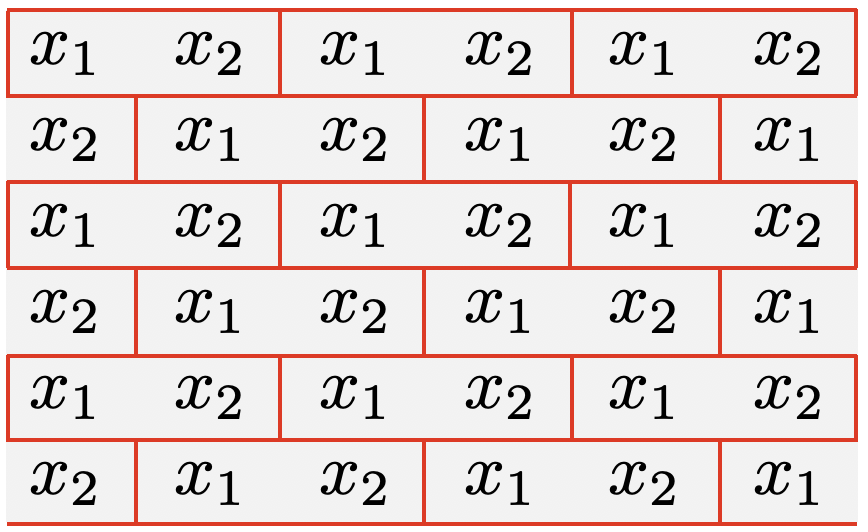
\includegraphics[width=1.0\textwidth]{HL2by1RelativePeriodicBlock}\\(a)
            \end{center}\end{minipage}
            \hskip 4ex
            \begin{minipage}[c]{0.46\textwidth}\begin{center}
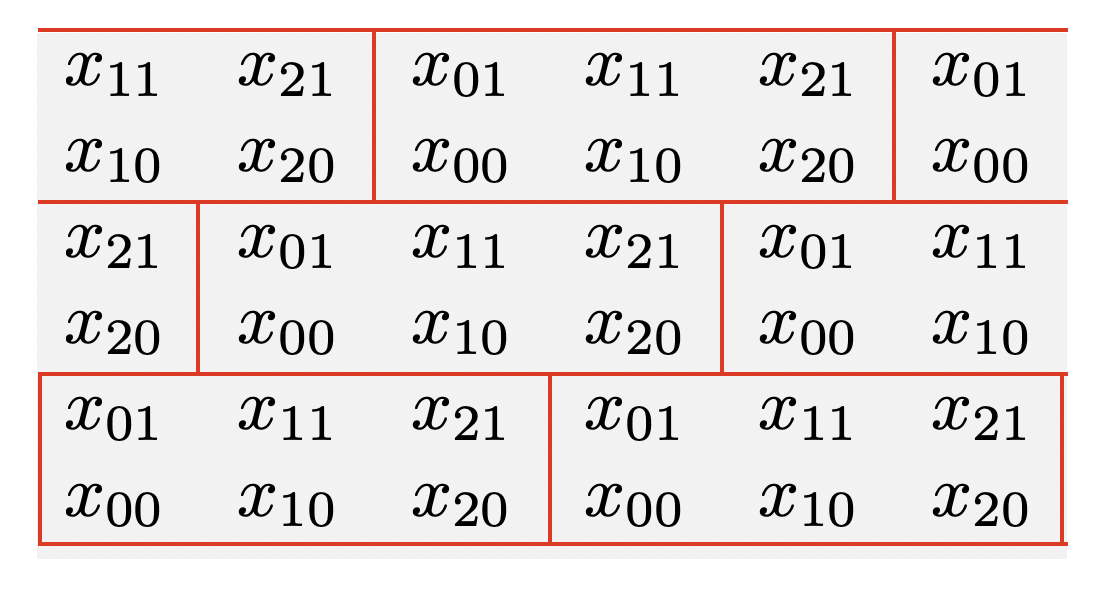
\includegraphics[width=1.0\textwidth]{HL2by3RelativePeriodicBlock}\\(b)
            \end{center}\end{minipage}
\end{center}
  \caption{\label{fig:2x1rpo}
Examples of $\LTS{}{}{}$ \twots\
together with their \spt\ Bravais lattice tilings \refeq{2DBravaisLattice}.
(a)
$\BravCell{2}{1}{1}$, basis vectors
$\mathbf{a}_1=\{2,0\}$ and $\mathbf{a}_2=\{1,1\}$;
(b)
$\BravCell{3}{2}{1}$, basis vectors
$\mathbf{a}_1=(3,0)$ and $\mathbf{a}_2=(1,2)$.
Rectangles enclose the Bravais cell and its Bravais lattice
translations.
}
\end{figure}
%%%%%%%%%%%%%%%%%%%%%%%%%%%%%%%%%%%%%%%%%%%%%%%%%%%%%%%%%%%%%%%




%\subsection{Admissible prime \twots}
%\label{s:prime2tAdmiss}
    \PC{2020-06-09}{explain \reftab{tab:LxTs}}

\begin{description}



	\HLpost{2020-06-09}{
\refFigs{fig:SpecialBravaisLatt}{fig:3x2rpo} are the plots of the
periodic \brick s by color. The three figures in
\reffig{fig:SpecialBravaisLatt} are the \brick s with periodicity
$\BravCell{1}{3}{0}$, $\BravCell{3}{1}{0}$ and $\BravCell{3}{1}{1}$,
which can show the periodicity of the space-\eqva, time-\eqva\ and
time-\reqva. \refFig{fig:3x2rpo} is the color coding of the periodic
blocks with periodicity $\BravCell{2}{1}{1}$, $\BravCell{3}{2}{1}$ and
$\BravCell{3}{2}{0}$.
	}

%%%%%%%%%%%%%%%%%%%%%%%%%%%%%%%%%%%%%%%%%%%%%%%%%%%%%%%%%%%%%
% HL 2020-06-09 siminos/figSrc/han/Mathematica/ColorBlock.nb
\begin{figure}\begin{center}
            \begin{minipage}[c]{0.25\textwidth}\begin{center}
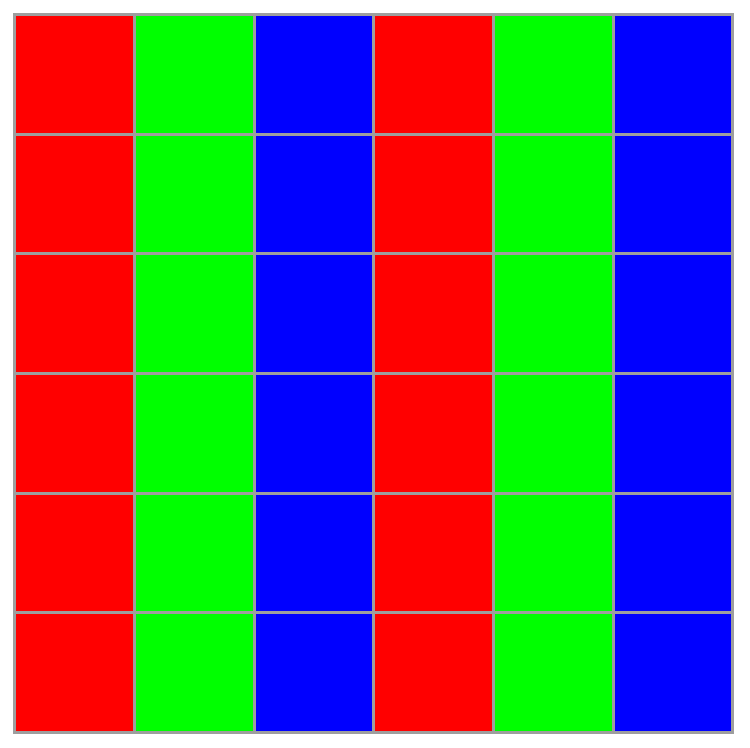
\includegraphics[width=1.0\textwidth]{HL310Block}\\(a)
            \end{center}\end{minipage}
            \hskip 4ex
            \begin{minipage}[c]{0.25\textwidth}\begin{center}
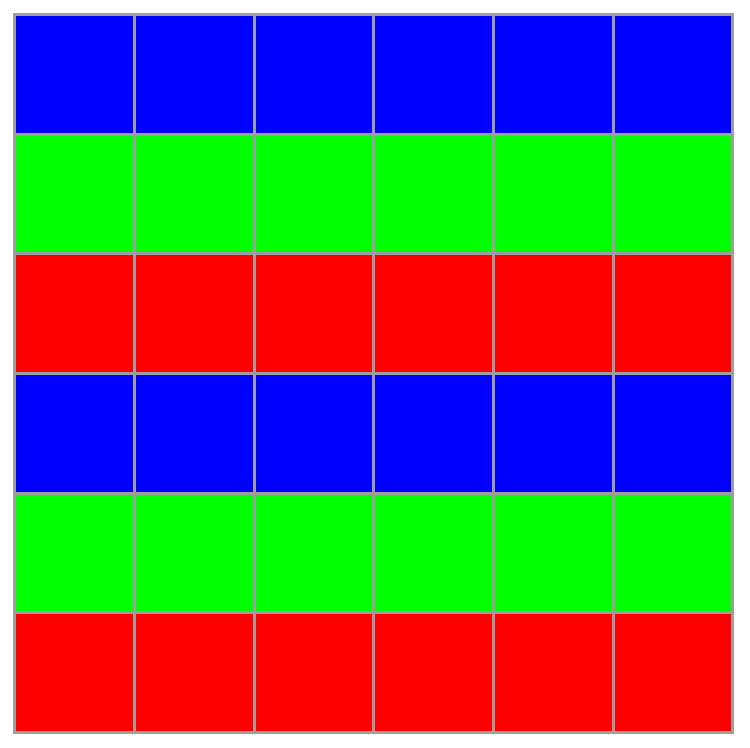
\includegraphics[width=1.0\textwidth]{HL130Block}\\(b)
            \end{center}\end{minipage}
            \hskip 4ex
            \begin{minipage}[c]{0.25\textwidth}\begin{center}
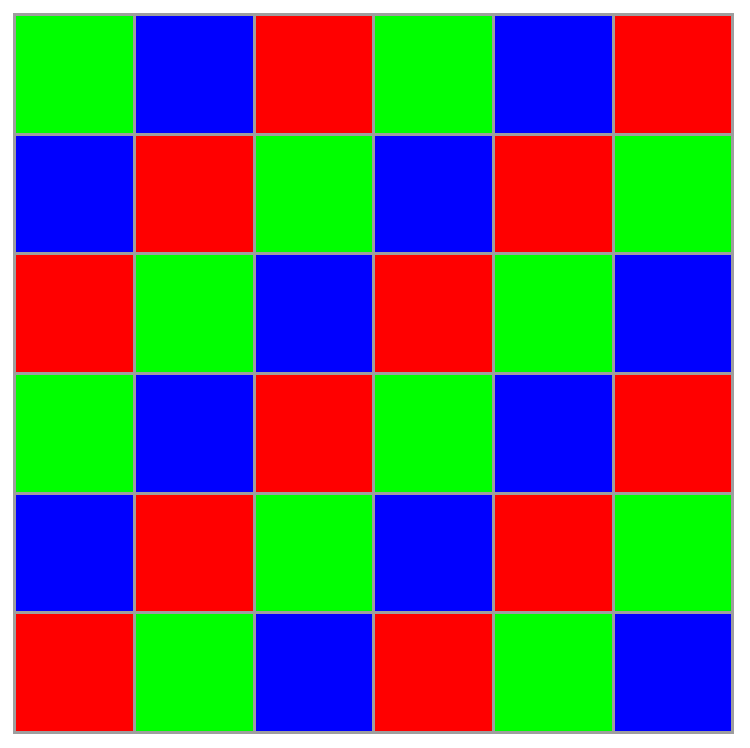
\includegraphics[width=1.0\textwidth]{HL311Block}\\(c)
            \end{center}\end{minipage}
\end{center}
  \caption{\label{fig:SpecialBravaisLatt}
Examples of $\LTS{}{}{}$ periodic \brick s
together with their \spt\ Bravais lattice tilings \refeq{2DBravaisLattice}.
(a)
$\BravCell{3}{1}{0}$, basis vectors
$\mathbf{a}_1=\{3,0\}$ and $\mathbf{a}_2=\{0,1\}$;
(b)
$\BravCell{1}{3}{0}$, basis vectors
$\mathbf{a}_1=\{1,0\}$ and $\mathbf{a}_2=\{0,3\}$;
(c)
$\BravCell{3}{1}{1}$, basis vectors
$\mathbf{a}_1=\{3,0\}$ and $\mathbf{a}_2=\{1,1\}$;
}
\end{figure}
%%%%%%%%%%%%%%%%%%%%%%%%%%%%%%%%%%%%%%%%%%%%%%%%%%%%%%%%%%%%%%%

%%%%%%%%%%%%%%%%%%%%%%%%%%%%%%%%%%%%%%%%%%%%%%%%%%%%%%%%%%%%%
% HL 2020-06-09 siminos/figSrc/han/Mathematica/ColorBlock.nb
\begin{figure}\begin{center}
            \begin{minipage}[c]{0.25\textwidth}\begin{center}
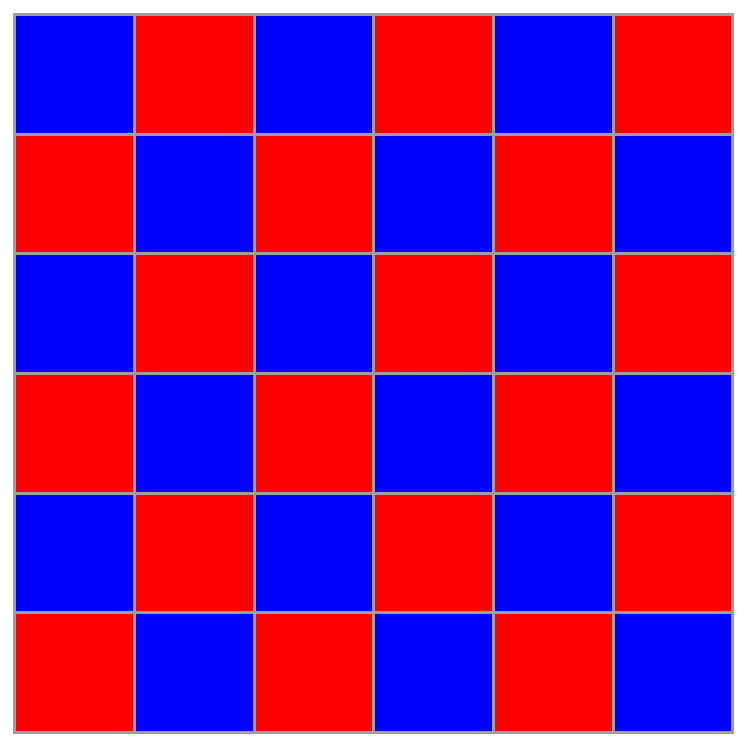
\includegraphics[width=1.0\textwidth]{HL211Block}\\(a)
            \end{center}\end{minipage}
            \hskip 4ex
            \begin{minipage}[c]{0.25\textwidth}\begin{center}
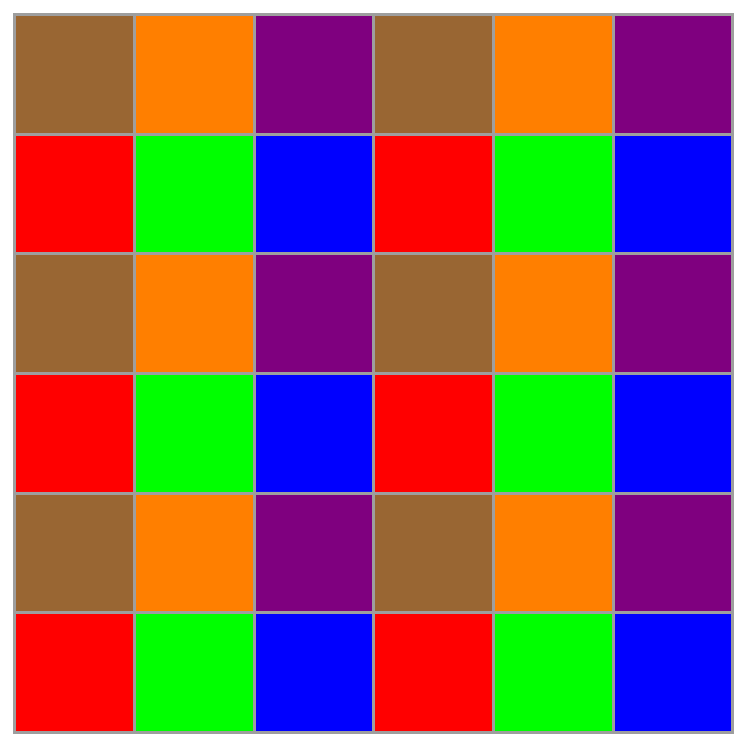
\includegraphics[width=1.0\textwidth]{HL320Block}\\(b)
            \end{center}\end{minipage}
            \hskip 4ex
            \begin{minipage}[c]{0.25\textwidth}\begin{center}
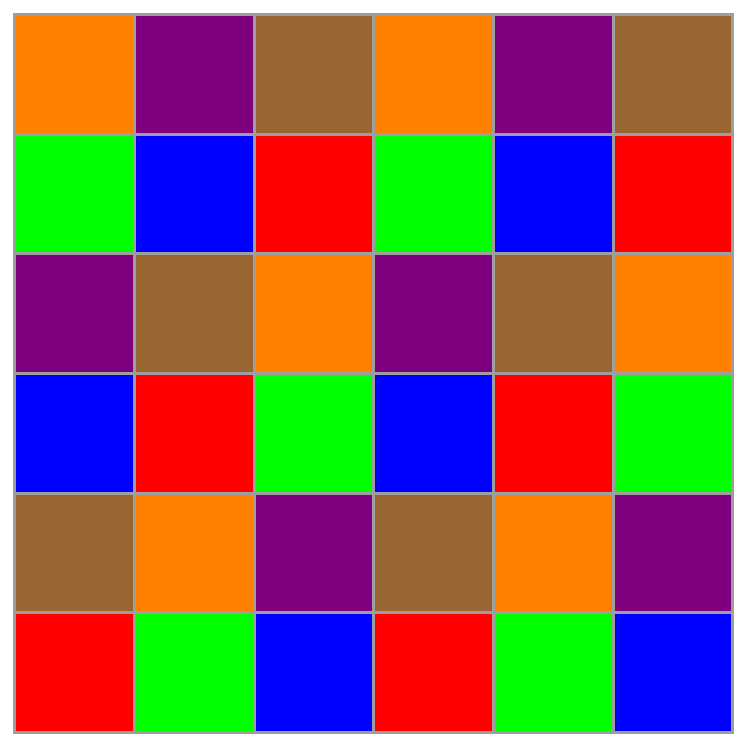
\includegraphics[width=1.0\textwidth]{HL321Block}\\(c)
            \end{center}\end{minipage}
\end{center}
  \caption{\label{fig:3x2rpo}
Examples of $\LTS{}{}{}$ periodic \brick s
together with their \spt\ Bravais lattice tilings \refeq{2DBravaisLattice}.
(a)
$\BravCell{2}{1}{1}$, basis vectors
$\mathbf{a}_1=\{2,0\}$ and $\mathbf{a}_2=\{1,1\}$;
(b)
$\BravCell{3}{2}{0}$, basis vectors
$\mathbf{a}_1=\{3,0\}$ and $\mathbf{a}_2=\{0,2\}$;
(c)
$\BravCell{3}{2}{1}$, basis vectors
$\mathbf{a}_1=\{3,0\}$ and $\mathbf{a}_2=\{1,2\}$;
}
\end{figure}
%%%%%%%%%%%%%%%%%%%%%%%%%%%%%%%%%%%%%%%%%%%%%%%%%%%%%%%%%%%%%%%

    \PCpost{2020-10-03}{
For periodic boundary conditions, the Laplacian $\Box$ in \refeq{OneCat}
and \refeq{2dCoupledCats} has a translational zero mode, $\lambda_0=0$,
corresponding to a constant eigenvector, so the matrix $\Box$ is
singular. That is the reason why our counting formulas
\refeq{1stChebGenF} and \reftab{tab:LxTs} have a prefactor $(s-2)$; in
the Laplacian limit the corresponding determinant has a zero eigenvalue,
and therefore vanishes.

A hyper-cubic lattice consists of $d$ intersecting one-dimensional
lattices, with Laplacian eigenvalues being the sums of the eigenvalues of
the Laplacian of the constituent one-dimensional lattices, hence for any
dimension there is only one zero eigenvalue, and only a single power of
the prefactor  $(s-2)$ in our counting formulas.
    }

    \PCpost{2019-11-23}{
We always reduce relative-shift symmetries, so I am not happy about the
$\BravCell{2}{1}{1}$ relative-periodic {\brick} \refeq{eq:block2x1rp} being
counted as the $\BravCell{2}{2}{0}$ \twot. We'll have to revisit symmetry
reduction...
    }


	\HLpost{2020-03-17}{
\emph{PrimeTiles.nb} generates all prime tiles that can tile a
larger tile. It gives
some not obvious results. For example, let the large tile be
$\BravCell{3}{2}{1}$, and consider the full-shift 9-symbol
$\BravCell{3}{2}{1}$ \brick s. The number $\BravCell{3}{2}{0}$ \brick s is
given by \refeq{catlattN3x2}. The program shows that the
$\BravCell{3}{2}{0}$ tile can only be tiled by $\BravCell{1}{1}{0}$,
$\BravCell{1}{2}{0}$ and $\BravCell{3}{1}{0}$ tiles. So we get the result in
\refeq{catlattN3x2}:
\[
N_{\BravCell{3}{2}{0}} = 9^{3\times2} =
88440\,\BravCell{3}{2}{0}+240\,\BravCell{3}{1}{0}
  +36\,\BravCell{1}{2}{0}+9\,\BravCell{1}{1}{0}
\,.
\]
For the full-shift the number of periodic \brick s is given
by the area of the larger tile, and number of $\BravCell{3}{2}{\tilt{}}$ \brick
s is the same for all $S$. But now
$\BravCell{3}{1}{0}$ tile cannot tile the $\BravCell{3}{2}{1}$ tile.
Instead, the $\BravCell{3}{2}{1}$ can be tiled by
$\BravCell{1}{1}{0}$, $\BravCell{3}{1}{2}$  and $\BravCell{1}{2}{0}$ tiles,
 \[
N_{\BravCell{3}{2}{1}} = 9^{3\times2} =
88440\,\BravCell{3}{2}{1}+ 240\,\BravCell{3}{1}{2}+36\,\BravCell{1}{2}{0}
   +9\,\BravCell{1}{1}{0}
\,.
\]
\emph{A priori} is not obvious that $\BravCell{3}{1}{2}$ tile can tile a
$\BravCell{3}{2}{1}$ tile. But if you stack $\BravCell{3}{1}{2}$ tile in the
shifted temporal direction by 2 then the left edge of the tile is shifted
by 4 in the spatial direction. With the spatial period being 3, shifted
by 4 in the spatial direction is same as shifted by 1. So the \bcs\ of
$\BravCell{3}{2}{1}$ tile are satisfied by the $\BravCell{3}{1}{2}$ tiles.
    }


\end{description}


%%%%%%%%%%%%%%%%%%%%%%%%%%%%%%%%%%%%%%%%%%%%%%%%%%%%%%%%%%%%%%%%%%%%%%%
%\printbibliography[heading=subbibintoc,title={References}]
